\documentclass[12pt]{article}
\usepackage{amsthm,amssymb,amsfonts,amsmath,amstext,systeme}
\usepackage{graphicx,float}
\marginparwidth 0pt
\oddsidemargin -1.2 truecm
\evensidemargin  0pt 
\marginparsep 0pt
\topmargin -2.2truecm
\linespread{1}
\textheight 25.8 truecm
\textwidth 18.5 truecm
\newenvironment{remark}{\noindent{\bf Remark }}{\vspace{0mm}}
\newenvironment{remarks}{\noindent{\bf Remarks }}{\vspace{0mm}}
\newenvironment{question}{\noindent{\bf Question }}{\vspace{0mm}}
\newenvironment{questions}{\noindent{\bf Questions }}{\vspace{0mm}}
\newenvironment{note}{\noindent{\bf Note }}{\vspace{0mm}}
\newenvironment{summary}{\noindent{\bf Summary }}{\vspace{0mm}}
\newenvironment{back}{\noindent{\bf Background}}{\vspace{0mm}}
\newenvironment{conclude}{\noindent{\bf Conclusion}}{\vspace{0mm}}
\newenvironment{concludes}{\noindent{\bf Conclusions}}{\vspace{0mm}}
\newenvironment{dill}{\noindent{\bf Description of Dill's model}}{\vspace{0mm}}
\newenvironment{maths}{\noindent{\bf Mathematics needed}}{\vspace{0mm}}
\newenvironment{inst}{\noindent{\bf Instructions}}{\vspace{0mm}}
\newenvironment{notes}{\noindent{\bf Notes }}{\vspace{0mm}}
\newenvironment{theorem}{\noindent{\bf Theorem }}{\vspace{0mm}}
\newenvironment{example}{\noindent{\bf Example }}{\vspace{0mm}}
\newenvironment{examples}{\noindent{\bf Examples }}{\vspace{0mm}}
\newenvironment{topics}{\noindent{\bf Topics}}{\vspace{0mm}}
\newenvironment{outcomes}{\noindent{\bf Expected Learning Outcomes}}{\vspace{0mm}}
\newenvironment{lemma}{\noindent{\bf Lemma }}{\vspace{0mm}}
\newenvironment{solution}{\noindent{\it Solution}}{\vspace{2mm}}
\newcommand{\ds}{\displaystyle}
\newcommand{\un}{\underline}
\newcommand{\bs}{\boldsymbol}

\begin{document}

\baselineskip 18 pt
\begin{center}
	{\large \bf HKDSE MATH M2 2015}\\
	\vspace{2 mm}

\end{center}
\vspace{0.05cm}

\begin{enumerate}
	\item \textbf{HKDSE Math M2 2015 Q1}\\
	Find $\displaystyle \frac{d}{dx} (x^5+4)$ from first principles. \\(4 marks)

	\item \textbf{HKDSE Math M2 2015 Q2}\\
	Let $y=x\sin{x} + \cos{x}$.  
	\begin{enumerate}
		\item [(a)]Find $\displaystyle\frac{dy}{dx}$ and $\displaystyle\frac{d^2y}{dx^2}$.
		\item [(b)]Let $k$ be a constant such that $x\displaystyle\frac{d^2y}{dx^2} + k\displaystyle\frac{dy}{dx} + xy = 0$ for all real values of $x$. Find the value of $k$.
	\end{enumerate}
	(5 marks)

	\item \textbf{HKDSE Math M2 2015 Q3}
	\begin{enumerate}
		\item [(a)]Find $\displaystyle\int \frac{1}{e^{2u}} \,du$. 
		\item [(b)]Using integration by substitution, evaluate $\displaystyle\int_1^9 \frac{1}{\sqrt{x}e^{2\sqrt{x}}}\,dx$. 
	\end{enumerate}
	(7 marks)

	\item \textbf{HKDSE Math M2 2015 Q4}
	\begin{enumerate}
		\item [(a)]Using integration by parts, find $\displaystyle\int x^2 \ln{x} \,dx $. 
		\item [(b)]At any point $(x,y)$ on the curve $\Gamma $, the slope of the tangent to $\Gamma$ is $9x^2 \ln{x}$. It is given that $\Gamma$ passes through the point $(1,4)$. Find the equation of $\Gamma$.  
	\end{enumerate}
	(7 marks)

	\item \textbf{HKDSE Math M2 2015 Q5}\\
	Solve the following systems of linear equations in real variables $x$, $y$, $z$:
	\begin{enumerate}
		\item [(a)]$\left\{
			\begin{matrix}
				x&+&y&+&z&=&2\\
				2x&+&3y&-&3z&=&4\\
			\end{matrix}\right.$;
		\item [(b)]$\left\{
			\begin{matrix}
				x&+&y&+&z&=&2\\
				2x&+&3y&-&3z&=&4\\
				3x&+&2y&+&kz&=&6\\
			\end{matrix}\right.$, where $k$ is a real constant.
	\end{enumerate}
	(6 marks)

	\item \textbf{HKDSE Math M2 2015 Q6}
	\begin{enumerate}
		\item [(a)]Let $M$ be a $3 \times 3$ real matrix such that $M^T = -M$, where $M^T$ is the transpose of $M$.\\
		Prove that $|M| = 0$.
		\item [(b)]Let $A = \begin{pmatrix}
			-1&a&b\\
			-a&-1&-8\\
			-b&8&-1\\
		\end{pmatrix}$, where $a$ and $b$ are real numbers. Denote the $3 \times 3$ identity matrix by $I$.
		\begin{enumerate}
			\item [(i)]Using (a), or otherwise, prove that $|A+I| = 0$. 
			\item [(ii)]Someone claims that $A^3 + I$ is a singular matrix. Do you agree? Explain your answer.
		\end{enumerate}
	\end{enumerate}
	(6 marks)

	\item \textbf{HKDSE Math M2 2015 Q7}
	\begin{enumerate}
		\item [(a)]Prove that $\sin^2{x}\cos^2{x} = \displaystyle\frac{1 - \cos{4x}}{8}$. 
		\item [(b)]Let $f(x) = \sin^4{x} + \cos^4{x}$. 
		\begin{enumerate}
			\item [(i)]Express $f(x)$ in the form $A\cos{Bx} + C$, where $A$, $B$ and $C$ are constants.
			\item [(ii)]Solve the equation $8f(x) = 7$, where $ 0\leq  x \leq \displaystyle\frac{\pi}{2}$.
		\end{enumerate}
	\end{enumerate}
	(7 marks)

	\item \textbf{HKDSE Math M2 2015 Q8}
	\begin{enumerate}
		\item [(a)]Using mathematical induction, prove that $\sin{\displaystyle\frac{x}{2}} \displaystyle\sum_{k = 1}^{n}\cos{kx} = \sin{\displaystyle\frac{nx}{2}}\cos{\displaystyle\frac{(n+1)x}{2}}$ for all positive integers $n$. 
		\item [(b)]Using (a), evaluate $\displaystyle\sum_{k = 1}^{567}\cos{\displaystyle\frac{k\pi}{7}}$.
	\end{enumerate}
	(8 marks)

	\item \textbf{HKDSE Math M2 2015 Q9}\\
	Define $f(x) = \displaystyle\frac{x^2+12}{x - 2}$ for all $x \neq 2$.  
	\begin{enumerate}
		\item [(a)]Find $f'(x)$. \\(2 marks)
		\item [(b)]Prove that the maximum value and the minimum value of $f(x)$ are $-4$ and $12$ respectively. \\(4 marks)
		\item [(c)]Find the asymptote(s) of the graph of $y = f(x)$. \\(3 marks) 
		\item [(d)]Find the area of the region bounded by the graph of $y = f(x)$ and the horizontal line $y = 14$.  \\(4 marks)
	\end{enumerate}


	\item \textbf{HKDSE Math M2 2015 Q10}\\
	$OAB$ is a triangle. $P$ is the mid-point of $OA$. $Q$ is a point lying on $AB$ such that $AQ : QB = 1 : 2$ while $R$ is a point lying on $OB$ such that $OR : RB = 3:1$. $PR$ and $OQ$ intersect at $C$. 
	\begin{enumerate}
		\item [(a)]		
		\begin{enumerate}
			\item [(i)]Let $t$ be a constant such that $PC : CR = t : (1-t)$.\\
				By expressing $\overrightarrow{OQ}$ in terms of $\overrightarrow{OA}$ and $\overrightarrow{OB}$, find the value of $t$. 
			\item [(ii)]Find $CQ:OQ$. 
		\end{enumerate}
		(7 marks)
		\item [(b)]Suppose that $\overrightarrow{OA} = 20\textbf{i} -6 \textbf{j} -12\textbf {k}$, $\overrightarrow{OB} = 16\textbf{i} -16 \textbf{j}$ and $\overrightarrow{OD} = \textbf{i} +3 \textbf{j} -6\textbf {k}$, where $O$ is the origin. Find
		\begin{enumerate}
			\item [(i)]the area of $\triangle OAB$, 
			\item [(ii)]the volume of tetrahedron $ABCD$.
		\end{enumerate}
		(5 marks)
	\end{enumerate}



	\item \textbf{HKDSE Math M2 2015 Q11}
	\begin{enumerate}
		\item [(a)]Let $\lambda$ and $\mu$ be real numbers such that $\mu - \lambda \neq 2$. Denote the $2 \times 2$ identity matrix by $I$.\\Define $\displaystyle A = \frac{1}{\lambda - \mu + 2} (I - \mu I + M)$ and $\displaystyle B = \frac{1}{\lambda - \mu + 2} (I +\lambda  I - M)$, \\where $M = \begin{pmatrix}
			\lambda & 1 \\ \lambda - \mu + 1 & \mu \\
		\end{pmatrix}$. 
		\begin{enumerate}
			\item [(i)]Evaluate $AB$, $BA$ and $A+B$. 
			\item [(ii)]Prove that $A^2 = A$ and $B^2 = B$. 
			\item [(iii)]Prove that $M^n = (\lambda + 1)^nA + (\mu -1)^n B$ for all positive integers $n$.
		\end{enumerate}
		(8 marks)
		\item [(b)]Using (a), or otherwise, evaluate $\begin{pmatrix}
			4&2\\0&6\\
		\end{pmatrix}^{315}$. \\(4 marks)
	\end{enumerate}
	
	\item \textbf{HKDSE Math M2 2015 Q12}
	\begin{enumerate}
		\item [(a)]In the figure, the curve $\Gamma$ consists of curve $AB$, the line segments $BC$ and $CO$, where $O$ is the origin, $B$ lies in the first quadrat and $C$ lies on the $x$-axis. The equations of $AB$ and $BC$ are $x^2-4y+8 = 0$ and $3x+y-9=0$ respectively.
			\begin{figure}[H]
				\centering
				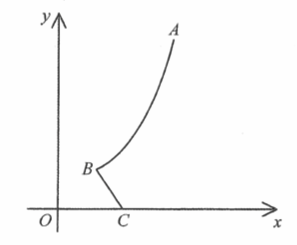
\includegraphics[width = .5\linewidth]{2015Figure1}
			\end{figure}
		\begin{enumerate}
			\item [(i)]Find the coordinates of $B$. 
			\item [(ii)]Let $h$ be the $y$-coordinate of $A$, where $h > 3$. A cup is formed by revolving $\Gamma$ about the $y$-axis. Prove that the capacity of the cup is $\pi(2h^2-8h+25)$.
		\end{enumerate}
		(7 marks)
		\item [(b)]A cup described in (a)(ii) is placed on a horizontal table. The radii of the base and the lip of the cup are 3 cm and 6 cm respectively.
		\begin{enumerate}
			\item [(i)]Find the capacity of the cup.
			\item [(ii)]Water is poured into the cup at a constant rate of $24\pi$ cm$^3$/s. Find the rate of change of the depth of water when the volume of water in the cup is $35\pi$ cm$^3$.
		\end{enumerate}
		(6 marks)
	\end{enumerate}
\end{enumerate}
\end{document}